\section{Diskussion}
\label{sec:Diskussion}

Die Versuchsdurchführung verlief ohne größere Probleme.
Einge Messwerte mussten zweimal aufgenommen werden, da das Oszilloskop nicht alle Spannungsverläufe gespeichert hat.
ZUnächst wurde eine Messung ohne Noise Generator durchgeführt, danach eine mit.
Die Messwerte und die dazugehörige Ausgleichskurve stellen ein zufriedenstellendes Ergebnis dar, da sich die Werte in der Nähe der Kosinus-Funktion befinden.
\noindent
Für die Eingangsspannungen wurden folgende Werte ermittelt:
\begin{align*}
    \text{ohne Noise Generator:}&  &U_{0,\text{ohne}} &= \SI{16.74 \pm 11.28}{\volt}, \\
    \text{mit Noise Generator:}&   &U_{0,\text{mit}}  &= \SI{ 3.17 \pm 1.18}{\volt}.
\end{align*}
Die eingestellte Eingangsspannung $U_\text{Ein}$ betrug $\SI{10}{\milli\volt}$, dadurch kann mit dem Verhältnis zwischen Ausgangsspannung und eingestellter Spannung der Verstärker bestimmt werden:
\begin{align*}
    \frac{U_{0,\text{ohne}}}{U_\text{Ein}} = 1674&  &\frac{U_{0,\text{mit}}}{U_\text{Ein}} = 317 .
\end{align*}
\\
\noindent
Bei der Untersuchung mithilfe der Photodioden müssen die Lichtverhältnisse berücksichtigt werden.
Die Deckenlampen wurden alle ausgeschaltet, dennoch kam genug Licht durch die Fenster hinein.
An diesen Umständen konnte nichts weiter geändert werden und hätten den Versuch stark beeinflussen können.
Die Messwerte zeigen aber gute Ergebnisse.
Die gewünschte $\sfrac{1}{r}$ Abhängigkeit ist gut zu sehen.
Da aber der Versuchsaufbau seine Grenzen hat und die Lichtverhältnisse auch nicht zu vernachlässigen sind,
konnte kein Extremwert aufgenommen werden, bei der die zu aufnehmende Spannung gegen Null geht.
Als maximaler Abstand und minimale Spannung wird somit $r = \SI{100}{\centi\metre}$ mit $U = \SI{126}{\milli\volt}$ aufgenommen.

%\section{Anhang}
%\begin{figure}
%    \centering
%    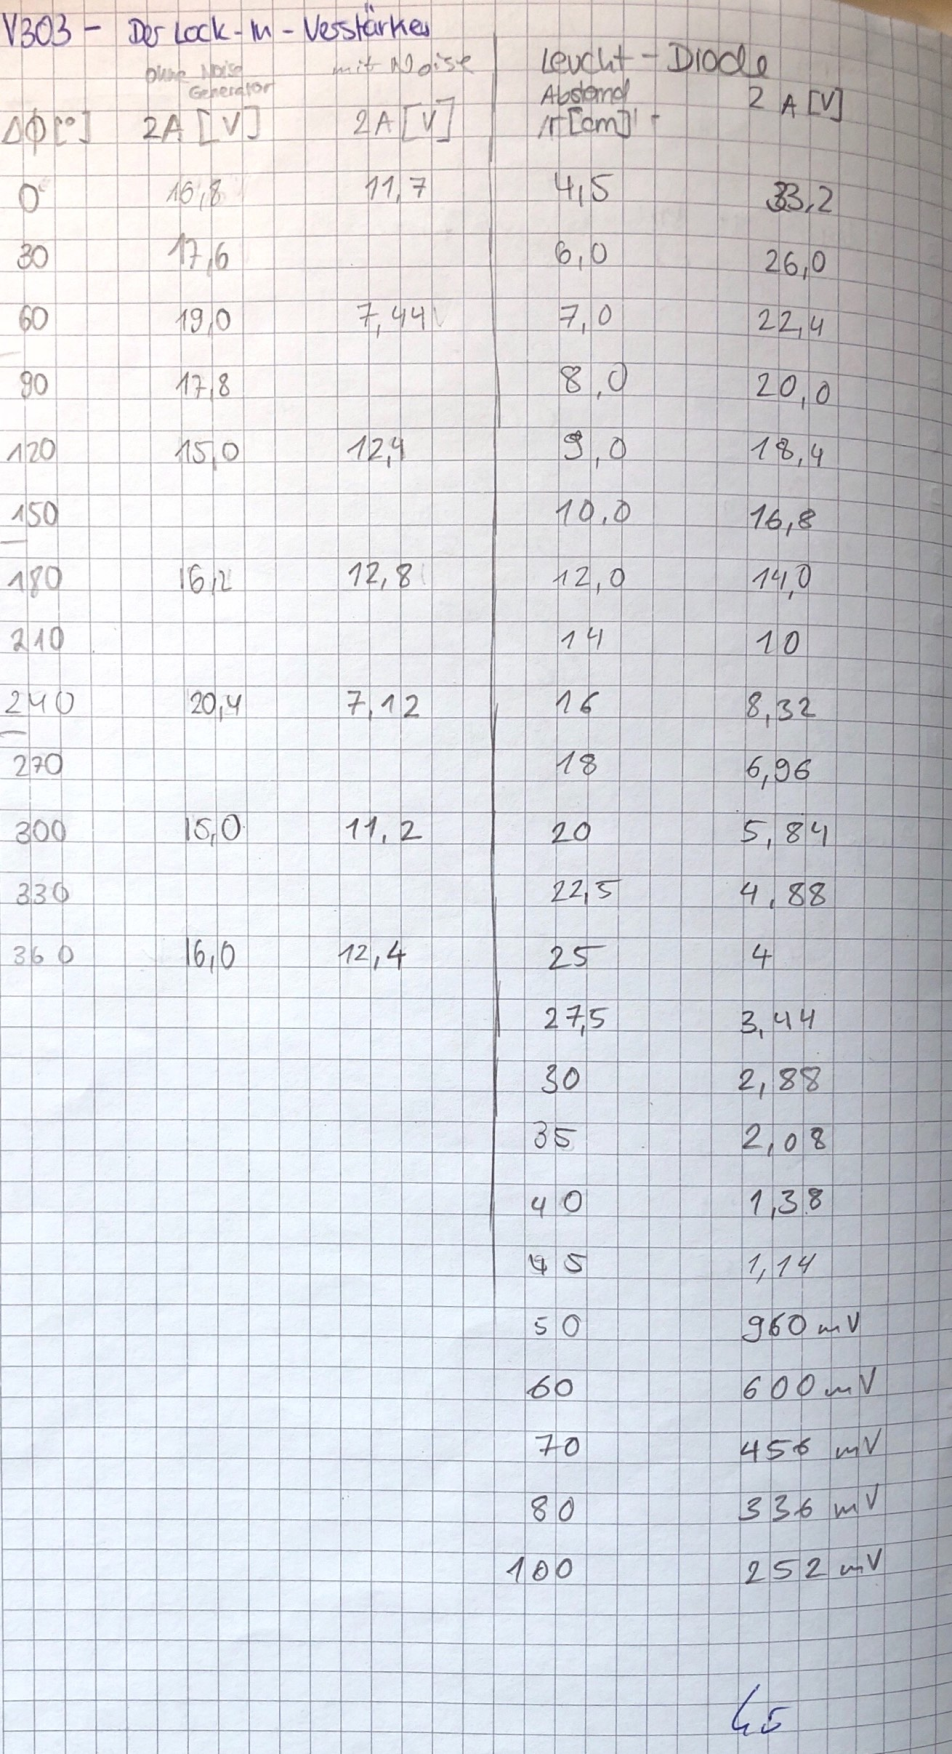
\includegraphics[width=\textwidth]{bilder/data_v303.pdf}
%    \caption{Die Originaldaten von der Versuchsdurchführung.}
%\end{figure}